\documentclass[paper=a4,twoside=false,fontsize=11pt,numbers=noenddot,version=first,bibliography=totoc,headsepline]{scrbook}

% Get the necessary packages for the document.
% Set to english language and utf8.
\usepackage[english]{babel}
\usepackage[utf8]{inputenc}

% Some packages for symbols we need within the tutorial.
\usepackage{dingbat}
\usepackage{marvosym}

% For the sourcecode.
\usepackage{listings}

% For the links etc.
\usepackage[pdfborder={0 0 0}]{hyperref}

% For the pdf-graphics.
\usepackage{graphicx}

% The steamroller tactics to fix figures and so on.
\usepackage{float}

% This is for tables which are to long to be shown on one page.
\usepackage{longtable}

% This package is for the directory tree structures
\usepackage{dirtree}

% We need this package for some color within the document.
\usepackage{color}

% This is the package for the margin-nodes.
\usepackage[color=white, bordercolor=white]{todonotes}

\usepackage{amsfonts}
\usepackage{setspace}
\usepackage{ae,aecompl}

\usepackage[automark]{scrpage2}

\usepackage[margin=0.5cm,indention=-3em,font={sf},labelfont={bf,sf},format=hang]{caption}
% Get the new commands we defined for this document.
% The name of Kieker, just for the case that the design of this should change.
\newcommand{\Kieker}{\textsf{Kieker}}

% The current version-string.
\newcommand{\version}{1.5-trunk}

% The single parts of Kieker and some files.
\newcommand{\KiekerMonitoringPart}{\textsf{Kieker.Monitoring}}
\newcommand{\KiekerAnalysisPart}{\textsf{Kieker.Analysis}}
\newcommand{\analysisJar}{kieker-analysis-\version.jar}
\newcommand{\monitoringJar}{kieker-monitoring-\version.jar}
\newcommand{\commonJar}{kieker-common-\version.jar}
\newcommand{\toolsJar}{kieker-tools-\version.jar}
\newcommand{\commonsLoggingJar}{commons-logging-1.1.1.jar}
\newcommand{\monitoringPropertiesFile}{kieker.monitoring.properties}
\newcommand{\analysisPropertiesFile}{kieker.analysis.properties}
\newcommand{\logFourJPropertiesFile}{log4j.properties}
\newcommand{\aopFile}{aop.xml}

% The complete url where to find Kieker.
\newcommand{\KiekerURL}{\url{http://sourceforge.net/projects/kieker/files}}

% This is how we call the kieker directory.
\newcommand{\KiekerDir}{kieker-\version{}}%{$<$KIEKER-DIR$>$}

% These commands are necessary to mark classes, methods and files within the document.
\newcommand{\class}[1]{\texttt{#1}}
\newcommand{\method}[1]{\textit{#1}}
\newcommand{\dir}[1]{\texttt{#1}}
\newcommand{\file}[1]{\texttt{#1}}

% TODO command for our document
\newcommand{\TODO}[1]{\todo[inline,color=green!40]{TODO: #1}}

% These commands are for notifying the reader about something important.
\newcommand{\marginbox}[1]{\todo[noline]{#1}}
\newcommand{\notify}{\marginbox{\huge{\rightpointleft}}}
\newcommand{\warning}{\marginbox{\huge{\Stopsign}}}


% The following commands set the listings for the different (programming) languages correctly.
% For the first they use all nearly the same settings.
\newcommand{\setListing}[4]{
\lstset{
language=#1,          
numbers=#2,
basicstyle=#3,       	% the size of the fonts that are used for the code
showspaces=false,               % show spaces adding particular underscores
showstringspaces=false,         % underline spaces within strings
showtabs=false,                 % show tabs within strings adding particular underscores
%frame=shadowbox,	                % adds a frame around the code
frame=lrtb,
rulesepcolor=\color{black},
tabsize=2,	                % sets default tabsize to 2 spaces
captionpos=t,                   % sets the caption-position to bottom
breaklines=true,                % sets automatic line breaking
breakatwhitespace=false,        % sets if automatic breaks should only happen at whitespace
title=\lstname,                 % show the filename of files included with \lstinputlisting; also try caption instead of title
escapechar={#4}
}
}
\newcommand{\setJavaCodeListing}{\setListing{Java}{left}{\sffamily\scriptsize}{}}
\newcommand{\setBashListing}{\setListing{Bash}{none}{\sffamily\scriptsize}{°}}
\newcommand{\setXMLListing}{\setListing{XML}{none}{\sffamily\scriptsize}{}}


\pagestyle{scrheadings}
\clearscrheadfoot

\ifoot[\hrule\sffamily Kieker \version{} User Guide]{\hrule\sffamily Kieker \version{} User Guide}
\ofoot[\hrule\sffamily\pagemark]{\hrule\sffamily\pagemark}

% Set the title and everything.
\titlehead{
  \begin{center}
    
\includegraphics[height=25mm]{./images/20120511-kieker-logo-1-6}\\
\href{http://kieker-monitoring.net}{\sffamily\Large http://kieker-monitoring.net}
  \end{center}
}

\title{%
\Huge\Kieker{} \version{} User Guide%
\footnote{\sffamily \textit{For guide lines on how to cite Kieker and this document, please see~Section~\ref{sec:ch1:citingKieker}.}}
}

\author{\sffamily Kieker Project%
% , and contributors
}
\date{\sffamily\today}
% \date{\sffamily May 19, 2011}
\publishers{\normalsize\sffamily

\begin{center}
\begin{tabular}{cc}
Kiel University & University of Stuttgart\\
Department of Computer Science & Institute of Software Technology\\
Software Engineering Group & Reliable Software Systems Group \\
Christian-Albrechts-Platz 4 & Universitätsstra\ss{}e 38\\
24118 Kiel, Germany & 70569 Stuttgart, Germany
\end{tabular}
\end{center}


%\flushleft
% 
\includegraphics[height=2.5cm]{./images/caulogo}\\[0.5ex]

}

\hypersetup
{%
pdftitle = {\Kieker{} \version{} User Guide},
pdfauthor = {Nils Ehmke, Andr\'e van Hoorn, and Reiner Jung}
% colorlinks = {true}
}

% Here we go.
\begin{document}
  % We want a table of contents separated from the rest of the text.
  \maketitle
  \setcounter{tocdepth}{1} % not deeper than section level
  {\sffamily\tableofcontents}

  \chapter{Introduction}\label{chp:Introduction}

	Modern software applications are often complex and have to fulfill a large set of functional and non-functional requirements. The internal behavior of such large systems cannot easily be determined on the basis of the source code. Furthermore, existing applications often lack sufficient documentation which makes it cumbersome to extend and change them for future needs. A solution to these problems can be dynamic analysis based on application-level monitoring, which allows to log the behavior of the application and to discover, for example, application-internal control flows, calling dependencies, and method response times.

	Dynamic analysis can help in detecting performance problems and faulty behavior, capacity planning, and many other areas. The Java-based \Kieker{} framework comes with tools and libraries for performance monitoring and dynamic software analysis \cite{KiekerICPE2012}. It has been designed for continuous monitoring in production systems inducing only a very low overhead. Monitoring adapters for other platforms, such as Visual Basic~6~(VB6), .NET, COBOL, and Perl are available upon request \footnote{\href{http://kieker-monitoring.net/support/}{Contact us} directly if you are interested in \Kieker{} support for these or other platforms}.  \\
	
	\noindent
	In 2011, Kieker was reviewed and accepted for distribution as part of the SPEC Research Group's repository of peer-reviewed tools for quantitative system evaluation and analysis. See \url{http://research.spec.org/projects/tools.html} for details.\\

	\NOTIFYBOX{In case that you are only interested in a quickstart example, you may want to skip directly to Chapter~\ref{chp:Quickstart-Example}.}
	
	\section{Kieker's Core Components}		
		Figure~\ref{fig:KiekerComponentDiagram} shows the framework's composition based on the two main components \KiekerMonitoringPart{} and \KiekerAnalysisPart{}. The \KiekerMonitoringPart{} component is responsible for program instrumentation, data collection, and logging. Its core is the \class{MonitoringController}. This part is explained in more detail in Chapter~\ref{chp:Kieker-Monitoring}. The component \KiekerAnalysisPart{} is responsible for reading, analyzing, and visualizing the monitoring data. Its core is the \class{AnalysisController} which manages the life-cycle of the pipe-and-filter architecture of analysis plugins, including monitoring readers and  analysis filters. This part is explained in more detail in Chapter~\ref{chp:Kieker-Analysis}.
		
		% This is the component diagram of Kieker (the satellite).
		\begin{figure}[H]\centering
			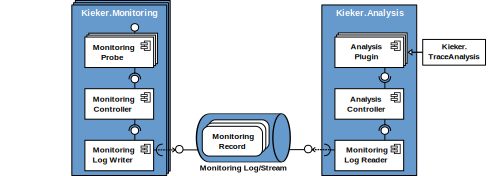
\includegraphics[width=0.81\textwidth]{images/kiekerComponentDiagram-woCloud-bw-w-record-newNames-withTraceAnalysis-colors}
			
			\caption{Overview of the framework components}
			\label{fig:KiekerComponentDiagram}
		\end{figure}
	
	\section{Download and Installation}
		
		The \Kieker{} download site\footnote{\KiekerDownloadURL{}} provides archives of the binary and source distribution, the Javadoc~API, as well as additional examples. The Java sources presented in this user guide, as well as pre-compiled binaries, are included in the \file{\exampleDir/} directory. The file \file{\mainJar{}} contains the \KiekerMonitoringPart{} and \KiekerAnalysisPart{} components, as well as the \KiekerTraceAnalysis{} tool. In addition to the \file{\mainJar{}} file, the \file{dist/} directory includes variants of this \file{.jar} files with integrated third-party libraries. Additional information on these \file{.jar} files and when to use them will follow later in this document.
		
	\section{Licensing}
		\Kieker{} is licensed under the Apache License, Version 2.0. You may obtain a copy of the license at \url{http://www.apache.org/licenses/LICENSE-2.0}. The \Kieker{} source and binary release archives include a number of third-party libraries. The \dir{lib/} directory of the release archives contains a \file{.LICENSE} file for each third-party library, pointing to the respective license text.	
		
	\section{Citing Kieker}\label{sec:ch1:citingKieker}
		When referencing Kieker resources in your publications, we would be happy if you respected the following guide lines:

		\begin{itemize}
			\item 
			When referencing the Kieker project, please cite our ICPE~2012~\cite{KiekerICPE2012} paper and/or our 2009 technical report~\cite{vanHoornRohrHasselbringWallerEhlersFreyKieselhorst2009TRContinuousMonitoringOfSoftwareServicesDesignAndApplicationOfTheKiekerFramework}. Also, you might want to add a reference to our web site (\url{http://kieker-monitoring.net/}) like~\cite{KiekerWebSite}. 
			\item 
			When referencing this user guide, e.g., when reprinting contents, please use a citation like~\cite{Kieker1.7UserGuide}.
		\end{itemize}

		\noindent At \url{http://kieker-monitoring.net/research/publications/} we provide entries for $\mathrm{B\scriptstyle IB}\!$\TeX{} and other bibliography systems.
		
	\section{Outline of this User Guide}
		The rest of this user guide is structured as followed. Chapter~\ref{chp:Quickstart-Example} contains a short quickstart example. In Chapter~\ref{chp:Kieker-Monitoring} we provide a detailed description of \KiekerMonitoringPart{} and its components, before presenting in Chapter~\ref{chp:Kieker-Analysis} the \KiekerAnalysisPart{} and its important parts. Various tools, which \Kieker{} already provides, can be found in Chapter~\ref{chp:Kieker-Tools}. The \hyperlink{hypertarget:appendix}{Appendix} finally includes additional resources, e.g., how to use the JMS writers and readers.
  \chapter{Quick Start Example}

This chapter provides a brief introduction to \Kieker{} based on a simple Bookstore example application. %
Section \ref{sec:example:downloadInstall} explains how to download and install \Kieker{}. The Bookstore application itself is introduced in Section \ref{sec:example:bookstore}, while the following Sections \ref{sec:example:monitoring} and \ref{sec:example:analysis} demonstrate how to use \Kieker{} for monitoring and analyzing the resulting monitoring data.

\section{Download and Installation}\label{sec:example:downloadInstall}

\Kieker{} can be downloaded from \KiekerURL. The web site provides zip/tar.gz archives of the \Kieker{} binary distribution as well as the corresponding \Kieker{} source code archives.

For this chapter, it is required to download and extract an archive containing \Kieker's binary distribution, e.g., \file{\binaryFileForDownload}. The extracted content has roughly the following directory structure:
% Note: The indention is not really necessary, but the tree is easier to understand in the tex-source.
\begin{figure}[H]
\begin{graybox}
\dirtree{%  
	.1 \DirInDirTree{\KiekerDir/}.
		.2 \DirInDirTree{bin/}\DTcomment{Call scripts for \Kieker{} tools}. 
			.3 \ldots. 
		.2 \DirInDirTree{doc/}\DTcomment{}. 
			.3 \DirInDirTree{tutorial/}. 
				.4 userguide.pdf\DTcomment{PDF file of this document}. 
				.4 source-example/\DTcomment{Source code of the examples in this document}. 
		.2 \DirInDirTree{dist/}\DTcomment{The \Kieker{} framework libraries}. 
			.3 \analysisJar. 
			.3 \commonJar. 
			.3 \monitoringJar. 
			.3 \toolsJar. 
		.2 \DirInDirTree{lib/}\DTcomment{Libraries required by \Kieker{}}. 
			.3 \ldots. 
		.2 \DirInDirTree{META-INF/}\DTcomment{Example configuration files}. 
			.3 \ldots. 
}
\end{graybox}
\caption{Directory structure and contents of \Kieker{}'s binary distribution}
\end{figure}

\section{Bookstore Example Application}\label{sec:example:bookstore}

The Bookstore application is a small sample application resembling a simple %
bookstore where a user can search for books in an online catalog. %
Figure~\ref{fig:bookstore:classAndSequenceDiagrams} \ldots

\begin{figure}[h]\centering
\subfigure[]{\label{fig:boostore:classdiagram}%
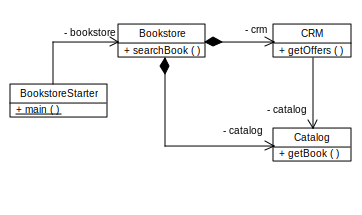
\includegraphics[scale=0.8]{images/kieker_bookstoreclassdiagram}%
}%
\subfigure[]{\label{fig:boostore:sequencediagram}%
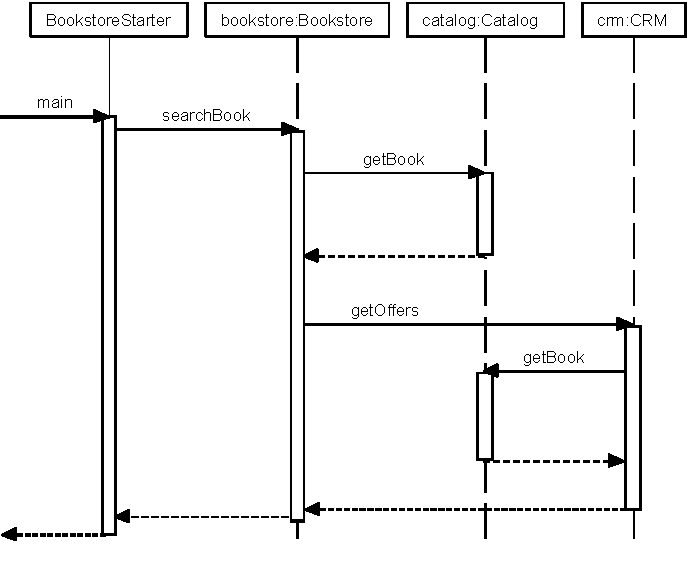
\includegraphics[scale=0.8]{images/kieker_SequenceDiagram-manually-changed}%
}
\caption{UML class diagram~\subref{fig:boostore:classdiagram} and %
sequence diagram~\subref{fig:boostore:classdiagram} of the Bookstore application}
\label{fig:bookstore:classAndSequenceDiagrams}
\end{figure}


\noindent Figure~\ref{Figure:PlainBookstoreExample} shows the directory structure of the application.

\begin{figure}[H]
\begin{graybox}
\dirtree{%
.1 \DirInDirTree{example/}. %\DTcomment{The root directory of the project}.
.2 \DirInDirTree{build/}\DTcomment{Directory for the Java class files}. 
.2 \DirInDirTree{src/}\DTcomment{The directory for the source code files}.
.3 \DirInDirTree{bookstoreApplication/}.
.4 Bookstore.java.
.4 BookstoreStarter.java.
.4 Catalog.java.
.4 CRM.java.  
}
\end{graybox}

\caption{The directory structure of the Bookstore application}
\label{Figure:PlainBookstoreExample}
\end{figure}

\noindent The following listings show the content of the source code files:

\setJavaCodeListing
\lstinputlisting[caption=Bookstore.java]{source-example/plain-example/src/bookstoreApplication/Bookstore.java}
\lstinputlisting[caption=CRM.java]{source-example/plain-example/src/bookstoreApplication/CRM.java}
\lstinputlisting[caption=Catalog.java]{source-example/plain-example/src/bookstoreApplication/Catalog.java}
\lstinputlisting[caption=BookstoreStarter.java]{source-example/plain-example/src/bookstoreApplication/BookstoreStarter.java}

\noindent The example can be compiled and executed as follows:
\setBashListing
% \begin{lstlisting}
nils@Laptop:~/example/$ javac src/mySimpleKiekerExampleManual/*.java -d build

nils@Laptop:~/example/$ java -classpath ./build/:./lib/commons-logging-1.1.1.jar\
                        mySimpleKiekerExampleManual.BookstoreMonitoringStarter 
\end{lstlisting}
% \WARNBOX{The default command-line interpreter of Windows doesn't support automatic file expansion. Therefore every single sourcefile has to be passed:
\begin{lstlisting}[caption=Commands to compile and run the Bookstore application]
#\lstshellprompt{}# javac src/bookstoreApplication/Bookstore.java 
        src/bookstoreApplication/BookstoreStarter.java 
        src/bookstoreApplication/Catalog.java 
        src/bookstoreApplication/CRM.java 
        -d build/

#\lstshellprompt{}# java -classpath build/ bookstoreApplication.BookstoreStarter 
\end{lstlisting}
%
%}

\noindent The following listing shows an example run of the application:
\begin{lstlisting}[caption=Example run of the ``plain'' application,label=lst:result-noinstr]
Bookstore.main: Starting request 0
Bookstore.main: Starting request 1
Bookstore.main: Starting request 2
Bookstore.main: Starting request 3
Bookstore.main: Starting request 4
\end{lstlisting}


\section{Monitoring}\label{sec:example:monitoring}
For the monitoring it is necessary to add some libraries from the \Kieker{}-framework to the example directory:
\begin{figure}[H]
\begin{graybox}
\dirtree{%
.1 \DirInDirTree{example/}. %\DTcomment{The root directory of the project}.
.2 \DirInDirTree{build/}\DTcomment{Directory for the Java class files}. 
.2 \newFileDirInDirTree{\DirInDirTree{lib/}}\DTcomment{Directory for the required libraries}.
.3 \newFileDirInDirTree{\monitoringJar}.
.3 \newFileDirInDirTree{\commonJar}.
.3 \newFileDirInDirTree{\commonsLoggingJar}.
.2 \DirInDirTree{src/}\DTcomment{The directory for the source code files}.
.3 \ldots.
}
\end{graybox}
\end{figure}

\noindent The \Kieker{} jar-files must be copied from the \dir{\KiekerDir/dist/} directory %
of the \Kieker{} release, as described in Section~\ref{sec:example:downloadInstall}. %
The file \file{commons-logging-1.1.1.jar} is included in \dir{\KiekerDir/lib/} %
and can also be copied from there.

The monitoring itself is done manually. Although this is not the strength of \Kieker\ it is pretty good for a quick start. Following listing shows how a method call is monitored:
\TODO{Imports?!\\ --- avh: ja, evtl. mit linerange, aber er bl\"oderweise nummeriert er so durch}
% Make sure that this listing will be modified, once the sourcecode changes!!!
% It must show the whole monitoring of the bookstorecall, from getting the first time to persisting of the record!!
\setJavaCodeListing
\lstinputlisting[linerange={11-29}, firstnumber=11, caption=Instrumentation of the \method{getBook()} call in Bookstore.java, label=listing:cuttingBookstore]%
{source-example/manual-monitoring/src/bookstoreApplication/Bookstore.java}
 
\noindent The time before and after a specific method call (in this case: \method{searchBook()}) is remembered. These information are stored in the so called operation execution record. Its (partially) layout can be seen in Figure \ref{Figure:OperationExecutionRecordClassDiagram}.

\begin{figure}[H]
\begin{centering}

\includegraphics[scale=1]{images/kieker_OperationExecutionRecord-notraceattributes}%
\caption{The class diagram of the operation execution record}
\label{Figure:OperationExecutionRecordClassDiagram}
\end{centering}
\end{figure}

\noindent The important attributes for now are:
\begin{compactitem}
\item \class{componentName:} The component (the class) in which the called method is.
\item \class{opName:} The called method.
% \item traceId: The trace id of the current trace we want to record. Due to the fact, that we follow only one trace, this is zero in all recordings.
\item \class{tin:} The time before the source code which should be measured.
\item \class{tout:} The time after the source code which should be measured.
\end{compactitem}

\quad\\

\noindent As an example, another method in \file{CRM.java} is monitored as well:

\setJavaCodeListing
\lstinputlisting[firstline=16, firstnumber=16, lastline=27, caption=Instrumentation of the \method{getBook()} call in CRM.java, label=listing:cuttingCRM]%
{source-example/manual-monitoring/src/bookstoreApplication/CRM.java}
The instrumented example can now be compiled and executed as follows:

\setBashListing 		
\begin{lstlisting}
nils@Laptop:~/example$ javac src/mySimpleKiekerExampleManual/*.java\
 -classpath ./lib/°\commonJar°:./lib/°\monitoringJar°:\
 -d build

nils@Laptop:~/example$ java\
-classpath ./build/:\
./lib/°\commonJar°:./lib/°\monitoringJar°:./lib/°\commonsLoggingJar°\
mySimpleKiekerExampleManual.BookstoreMonitoringStarter 
\end{lstlisting}
	

\begin{lstlisting}[caption=Commands to compile and run the instrumented Bookstore under Windows,label=lst:bookstoreStarterWin]
#\lstshellprompt{}# mkdir build
#\lstshellprompt{}# javac src\bookstoreApplication\*.java -classpath lib\#\mainJar# -d build\

#\lstshellprompt{}# java -classpath build\;
       lib\#\mainJar#;
       lib\#\commonsLoggingJar#
       bookstoreApplication.BookstoreStarter 
\end{lstlisting}


\WARNBOX{%
The default command-line interpreter of Windows doesn't support automatic %
file expansion. Therefore every single source file has to be passed, as %
shown in Listing~\ref{lst:bookstoreStarterWin}. %
Also, it is necessary to separate the different elements of the classpath with %
a semicolon instead of a colon.}

\noindent If everything worked correctly, there should now be a new directory with the %
name \dir{tpmon-20100727-181422131-UTC/} (just with another timestamp) in the default %
temporary directory (under Linux this should be \dir{/tmp/}; under Windows %
\dir{C:\textbackslash{}temp\textbackslash{}}). In this directory, there should be a file with the extension %
\dir{.dat} which contains the recorded information from the source code and %
a file named \dir{tpmon.map} which contains information about the types of the %
monitoring records. %
The Listings~\ref{listing:exampledat} and \ref{listing:examplemap} show example %
contents. 
\begin{figure}[H]
\begin{graybox}
\dirtree{%
.1 \DirInDirTree{/tmp/}.
.2 \DirInDirTree{tpmon-20100727-181422131-UTC/}.
.3 tpmon.map.
.3 tpmon-20100727-181422234-UTC-Thread-2.dat.
}
\end{graybox}
\end{figure}

\setBashListing
\lstinputlisting[caption=tpmon-20100727-181422234-UTC-Thread-2.dat (excerpt), firstline=1, lastline=3, label=listing:exampledat]%
{ch2-quickstart-example/tpmon-20100727-181422131-UTC/tpmon-20100727-181422234-UTC-Thread-2.dat}

\lstinputlisting[caption=tpmon.map, label=listing:examplemap]%
{ch2-quickstart-example/tpmon-20100727-181422131-UTC/tpmon.map}

\noindent The \file{.dat}-file is saved as a CSV-file (\textbf{C}omma \textbf{S}eparated \textbf{V}alues), meaning that it can be opened with Microsoft Excel or OpenOffice.org Calc. It would be possible to visualize the stored data with the help of these programs, but we will show in Section \ref{sec:example:analysis} how to use \KiekerAnalysisPart\ to read and process the files.

\section{Analysis}\label{sec:example:analysis}
As mentioned in the beginning of this chapter, it is shown how a simple consumer is programmed before starting the analysis. Therefore we need some new files:
\begin{figure}[H]
\begin{graybox}
\dirtree{%  
.1 \DirInDirTree{example/}. 
.2 \DirInDirTree{build/}\DTcomment{Directory for the Java class files}. 
.2 \DirInDirTree{lib/}\DTcomment{Directory for the required libraries}.
.3 \ldots. 
.3 \newFileDirInDirTree{\analysisJar}.
.2 \DirInDirTree{src/}\DTcomment{The directory for the source code files}.
.3 \DirInDirTree{bookstoreApplication/}.
.4 \ldots. 
.4 \newFileDirInDirTree{BookstoreAnalysisStarter.java}.
.4 \newFileDirInDirTree{Consumer.java}.
}
\end{graybox}
\end{figure}

\noindent The new jar-file can again be found in \dir{\KiekerDir/dist}. Listing \ref{listing:Consumer} shows the content of the new created \dir{Consumer.java}. It implements the \class{IMonitoringRecordConsumerPlugin} and overrides the necessary methods so that it can later be used by the analysis component of \Kieker. In this case the component gets a maximal response time within the constructor which will later be used to check whether a recorded method call replied fast enough or not. If the method call needed more time to response that the maximal allowed response time, it will be written directly to the error stream.\\
The methods \method{terminate} and \method{execute} don't do anything due to the fact that the consumer doesn't need any initialization. If the consumer would for example use threads then these methods would be the correct location to start and stop them.

\setJavaCodeListing       
\lstinputlisting[caption=Consumer.java, label=listing:Consumer]{source-example/manual-monitoring/src/bookstoreApplication/Consumer.java}

\noindent Now, we have to create the file \dir{BookstoreAnalysisStarter.java} to analyze our recorded information. 

The analysis consists thereby of the following steps:
\begin{compactenum}
\item Create a new instance (or more) of the class \class{AnalysisInstance}.
\item Register the plugins which should evaluate the records.
\item Register exactly one reader to read the stored information.
\item Start the analysis instance.
\end{compactenum}

\setJavaCodeListing       
\lstinputlisting[caption=BookstoreAnalysisStarter.java]{source-example/manual-monitoring/src/bookstoreApplication/BookstoreAnalysisStarter.java}
As can be seen, the application expects the output directory from the earlier monitoring run (see Section \ref{sec:example:monitoring}) as argument, which must be passed manually. Following listings show again the course of action:
\setBashListing 		
\begin{lstlisting}[caption=Commands to compile and run the analysis under \UnixLikeSystems{},label=lst:bookstoreAnalysisStarterLinux] 			
#\lstshellprompt{}# mkdir build
#\lstshellprompt{}# javac src/kieker/examples/userguide/ch2bookstore/manual/*.java 
        -classpath lib/#\mainJarEMF# -d build/

#\lstshellprompt{}# java -classpath build/:lib/#\mainJarEMF#
       kieker.examples.userguide.ch2bookstore.manual.BookstoreAnalysisStarter 
       /tmp/kieker-20120402-163314855-UTC-myHost-KIEKER-SINGLETON
\end{lstlisting}		
\begin{lstlisting}[caption=Commands to compile and run the analysis under Windows,label=lst:bookstoreAnalysisStarterWin]
#\lstshellprompt{}# mkdir build
#\lstshellprompt{}# javac src\kieker\examples\userguide\ch2bookstore\manual\*.java 
        -classpath lib\#\mainJarEMF# -d build\

#\lstshellprompt{}# java -classpath build\;lib\#\mainJarEMF#
       kieker.examples.userguide.ch2bookstore.manual.BookstoreAnalysisStarter 
       C:\Temp\kieker-20130910-120352847-UTC-myHost-KIEKER-SINGLETON
\end{lstlisting}	

	
It should be ensured that the application gets the correct path from the monitoring run. 

If everything worked correctly, the consumer should write something on the outputstream for every record it gets. A possible display of the run can be found in the appendix of this tutorial. 
  \chapter{Kieker Monitoring}\label{chp:Kieker-Monitoring}
	\section{The Concept behind the Monitoring}
		\subsection{Data Flow}
		\subsection{Monitoring Components}
	\section{How to Monitor Applications}
		\subsection{Manual Probes}
		\subsection{Aspect Oriented Probes}
		\subsection{Monitoring within Java EE Applications}
			\subsubsection{Spring Probes}
			\subsubsection{Aspect Oriented Probes}
			\subsubsection{SOAP Interceptors}
		\subsection{Periodic Samplers}
			\subsubsection{Sigar}
	\section{Creating and Controlling the Monitoring}
		\subsection{Time Sources}
		\subsection{Adaptive Monitoring}
		\subsection{JMX MBean Access}
	\section{Development of own Monitoring Components}
		\subsection{Records}
		\subsection{Probes}
		\subsection{Writers}
  \chapter{Kieker Analysis}\label{chp:Kieker-Analysis}
	\section{The Concept behind the Analysis}
		\subsection{Data Flow}
		\subsection{Analysis Components}
	\section{Creating and Controlling the Analysis}
	\section{Development of own Analysis Components}
		\subsection{Readers}
		\subsection{Filters}
		\subsection{Repositories}
  \chapter{Kieker Tools}\label{chp:Kieker-Tools}
	\section{Trace Analysis}
		\subsection{Textual Trace and Equivalence Class Representations}
			\subsubsection{Execution Traces}
			\subsubsection{Message Traces}
			\subsubsection{Trace Equivalence Classes}
		\subsection{Sequence Diagrams}
			\subsubsection{Deployment-Level Sequence Diagrams}
			\subsubsection{Assembly-Level Sequence Diagram}
		\subsection{Call Trees}
			\subsubsection{Trace Call Trees}
			\subsubsection{Aggregated Call Trees}
		\subsection{Dependency Graphs}
			\subsubsection{Container Dependency Graphs}
			\subsubsection{Component Dependency Graphs}
			\subsubsection{Operation Dependency Graphs}
			\subsubsection{Response Times}
		\subsection{HTML Output of the System Model}	
			
	\section{Kieker WebGUI}
			
		The \KiekerWebGUI{} is a JavaEE-based web application to assemble, control, and observe Kieker analyses. Although currently still in the beta state, it already provides a user and project management, a graphical editor, and a control interface for analyses. A cockpit, which can be used, for example, for the realtime monitoring of applications, is currently under development.

		Like \Kieker{}, the \KiekerWebGUI{} project is licensed under the Apache License, Version 2.0. 
		
		\subsection{Download and Installation}
		
			The application can be downloaded as \file{.zip} and \file{.tar.gz} file on the \Kieker{} website under \url{http://kieker-monitoring.net/download/}. Once downloaded and extracted, the directory structure in Figure~\ref{fig:webgui-binary-layout} should be visible. In order to start the web application on Jetty, a lightweight web server, execute the suitable start script for your operation system in the \file{bin} directory. Depending on the system, the start procedure can take several minutes. Once started, the web application is available under \url{http://localhost:8080/Kieker.WebGUI/login}.
			
			\begin{figure}[h!]
				\begin{graybox}
					\dirtree{%
						.1 \DirInDirTree{\KiekerWebGUIDir/}.
							.2 \DirInDirTree{bin/}\DTcomment{Start scripts for the \KiekerWebGUI{}}.
								.3 Kieker.WebGUI.bat.
								.3 Kieker.WebGUI.sh.
							.2 \DirInDirTree{lib/}\DTcomment{Libraries required to start the \KiekerWebGUI{}}.
								.3 \ldots.
							.2 \DirInDirTree{target/}.
								.3 Kieker.WebGUI-1.7.war\DTcomment{The web application archive containing the \KiekerWebGUI{}}.
					}
				\end{graybox}
				
				\caption{Directory structure and contents of \KiekerWebGUI{}'s binary distribution}
				\label{fig:webgui-binary-layout}
			\end{figure}
			
			\noindent
			The web application provides per default three users (Table~\ref{tab:webgui-default-users}), which can be used to log in. Further users can be created when logged in as administrator.
			
			\begin{table}[h!]
				\center
				
				\begin{tabular}{|c|c|}
					\hline
					Username & Password\\
					\hline
					\hline
					guest    & kieker\\
					user     & kieker\\
					admin    & kieker\\
					\hline
				\end{tabular}
			
				\caption{Default users in the \KiekerWebGUI{}}
				\label{tab:webgui-default-users}
			\end{table}
			
		\subsection{Quickstart Example}
		
			\NOTIFYBOX{
				For the quickstart example it is assumed that you are already logged into the \KiekerWebGUI{}, either as an user or as an administrator. You should also enable javascript and cookies, as both is necessary for the functionality of the application. 
			}
		
		\subsection{Detailed Introduction}
			
	\section{Supporting Tools}
		\subsection{Replay Monitoring Logs}
		
			Replays filesystem monitoring logs created by \KiekerMonitoringPart{}. Example applications are:
			\begin{compactitem}
				\item 
				Merging multiple directories containing monitoring data into a single output directory. 
				\item 
				Importing a filesystem monitoring log to another monitoring log, e.g., a database. Therefore, an appropriate \KiekerMonitoringPart{} configuration	file must be passed to the script.
				\item 
				Replaying a recorded filesystem monitoring log in real-time in order to simulate incoming monitoring data from a running system, e.g., via JMS. 
			\end{compactitem}

			\

			\noindent Main-class: {\small \class{kieker.tools.logReplayer.FilesystemLogReplayerStarter}}

			\paragraph*{Usage}\

				\setTextListing
				\begin{lstlisting}[gobble = 10]
					usage: kieker.tools.logReplayer.FilesystemLogReplayerStarter
					 --c,--monitoring.configuration <\path\to\monitoring.properties>
							Configuration to use for the Kieker monitoring instance

					 --i,--inputdirs <dir1 ... dirN>
							Log directories to read data from

						--ignore-records-after-date <yyyyMMdd-HHmmss>
							Records logged after this date (UTC timezone) are ignored
							(disabled by default).

						--ignore-records-before-date <yyyyMMdd-HHmmss>
							Records logged before this date (UTC timezone) are ignored
							(disabled by default).

					 --k,--keep-logging-timestamps <true|false>
							Replay the original logging timestamps (defaults to true)?)

					 --n,--realtime-worker-threads <num>
							Number of worker threads used in realtime mode (defaults to 1).

					 --r,--realtime <true|false>
							Replay log data in realtime?. 
				\end{lstlisting}

			\paragraph*{Example}\

				\noindent The following command replays the monitoring testdata included in the binary release to another directory:

				\setTextListing
				\begin{lstlisting}[gobble = 10, caption=Execution under UNIX-like systems]
					$\lstshellprompt{}$ $\textbf{bin/logReplay.sh}$
					  $\textbf{-\,-inputdirs}$ $\distributedTestdataDirDistro$ 
					  $\textbf{-\,-keep-logging-timestamps}$ $true$ 
					  $\textbf{-\,-realtime}$ $false$
				\end{lstlisting}
				\begin{lstlisting}[gobble = 10, caption=Execution under Windows]
					$\lstshellprompt{}$ $\textbf{logReplay.bat}$
					  $\textbf{-\,-inputdirs}$ $\distributedTestdataDirDistroWin$ 
					  $\textbf{-\,-keep-logging-timestamps}$ $true$ 
					  $\textbf{-\,-realtime}$ $false$
				\end{lstlisting}
		
		\subsection{Convert Monitoring Timestamps}
		
			The script converts \KiekerMonitoringPart{} logging timestamps, representing the number of nanoseconds since 1~Jan 1970 00:00 UTC, to a human-readable textual representation in the UTC and local timezones.\\
			
			\noindent Main-class: {\small \class{kieker.tools.loggingTimestampConverter.LoggingTimestampConverterTool}}

			\paragraph*{Usage}\

				\setTextListing
				\begin{lstlisting}[gobble = 10]
					usage: kieker.tools.loggingTimestampConverter.LoggingTimestampConverterTool -t
						   <timestamp1 ... timestampN>
					 --t,--timestamps <timestamp1 ... timestampN>
							List of timestamps (UTC timezone) to convert
				\end{lstlisting}

			\paragraph*{Example}\

				\noindent
				The following listing shows the command to convert two logging timestamps as well as the resulting output.

				\setTextListing
				\begin{lstlisting}[gobble = 10, caption=Execution under UNIX-like systems]
					$\lstshellprompt{}$ $\textbf{bin/convertLoggingTimestamp.sh}$ $\textbf{-\,-timestamps}$ 1283156545581511026 1283156546127117246 
					1283156545581511026: Mo, 30 Aug 2010 08:22:25 +0000 (UTC) (Mo, 30 Aug 2010 10:22:25 +0200 (local time))
					1283156546127117246: Mo, 30 Aug 2010 08:22:26 +0000 (UTC) (Mo, 30 Aug 2010 10:22:26 +0200 (local time))
				\end{lstlisting}

				\begin{lstlisting}[gobble = 10, caption=Execution under Windows]
					$\lstshellprompt{}$ $\textbf{convertLoggingTimestamp.bat}$ $\textbf{-\,-timestamps}$ 1283156545581511026 1283156546127117246 
					1283156545581511026: Mo, 30 Aug 2010 08:22:25 +0000 (UTC) (Mo, 30 Aug 2010 10:22:25 +0200 (local time))
					1283156546127117246: Mo, 30 Aug 2010 08:22:26 +0000 (UTC) (Mo, 30 Aug 2010 10:22:26 +0200 (local time))
				\end{lstlisting}
		
		\subsection{KAX Viz}
		
			The KAX Viz tool visualizes a \KiekerAnalysisPart{} pipe-and-filter configuration file (\file{.kax} file).\\

			\noindent Main-class: {\small \class{kieker.tools.KaxViz}}

			\paragraph*{Usage}\

				\setTextListing
				\begin{lstlisting}[gobble = 10]
					usage: kieker.tools.KaxViz -i <filename> [-svg <filename>]
					 --i,--input <filename>
							the analysis project file (.kax) loaded

					 --svg <filename>
							name of svg saved on close
				\end{lstlisting}
		
		\subsection{KAX Runner}
		
			The KAX Runner tool executes a \KiekerAnalysisPart{} pipe-and-filter configuration file (\file{.kax} file). \\

			\noindent Main-class: {\small \class{kieker.tools.KaxRun}}

			\paragraph*{Usage}\

				\setTextListing
				\begin{lstlisting}[gobble = 10]
					usage: kieker.tools.KaxRun -i <filename>
					 --i,--input <filename>
							the analysis project file (.kax) loaded
				\end{lstlisting}	
			
	\section{TSLib \& OPAD}
	
  \appendix
	\phantomsection
	\addcontentsline{toc}{chapter}{Appendix}\hypertarget{hypertarget:appendix}{}
	\addtocontents{toc}{\protect\setcounter{tocdepth}{-1}}

	\chapter{JMS}
		\section{OpenJMS}
		\section{ActiveMQ}
		\section{HornetQ}
		
	\chapter{Sigar}
  
  % suppress appendix chapters in toc:
  \addtocontents{toc}{\protect\setcounter{tocdepth}{0}}

\bibliographystyle{abbrvnatAvanhoorn} % alpha
\bibliography{bibliography}
\end{document}

